\section{Experiments}
\label{sec:experiments}

\subsection{Experimental Setup}
\label{sec:setup}

We evaluate \ModelClaudeOpus, \ModelAstra, \ModelDeepSeek, \ModelGemini, \ModelGLM, and \ModelKimi\ using the platform's standard research harness. Models develop strategies on the 2022--2023 research period, and their frozen programs are assessed on the sealed year 2024. Each independent research attempt has a budget of 500,000 model tokens.

We compare two research settings. \textbf{One-shot} asks the model to produce a complete strategy without research-performance feedback. The harness permits corrections to invalid proposals. \textbf{Iterative research} allows the model to revise candidates using return, signal-quality, coverage, and execution-error feedback, with at most five candidate evaluations. The model then commits one completed strategy for assessment. Both settings use the data access and financial evaluation defined in Section~\ref{sec:benchmark}.

The main comparison follows the leaderboard selection: for each model and setting, we report the retained entry with the highest overall score among eligible submissions. Existing retained entries are used when scores tie. Each row contains the scores and financial metrics of that same strategy. Individual submissions remain available for the supplementary analysis. We include our closed-source strategy Kelper-1 as a professional reference and compare returns against the equal-weight market reference over the same assessment period. The market reference is gross of trading costs.

We report the overall score, research-period and assessment-period scores, and the assessment-period annualized return (ARR), excess ARR, long-only Sharpe ratio, and maximum drawdown (MDD). Excess ARR is the difference from the market reference, expressed in percentage points. The errors-only control described in Section~\ref{sec:feedback_effect} uses the same research budget and evaluation rules while withholding performance feedback.

\subsection{Overall Performance}
\label{sec:main}

% Keep the main results and their NAV curves together on the page.
\begin{table*}[!t]
    \begin{minipage}{\linewidth}
        \begin{table}[H]
  \caption{Main comparison under the \BenchmarkName\ contract. Every arm uses the same markets, seeds, proposal budget, expression language, factor-fusion model, portfolio simulator, and confirmation evaluator. Factor predictive power and strategy performance are reported separately, with validity and token usage retained as search diagnostics. Values are placeholders pending the final frozen campaigns; the released version will additionally report each market--seed cell.}
  \label{tab:main}
  \centering
  \small
  \begin{tabular}{lrrrrrrr}
    \toprule
    Arm & \multicolumn{2}{c}{\textbf{Factor Predictive Power}} & \multicolumn{3}{c}{\textbf{Strategy Performance}} & \multicolumn{2}{c}{\textbf{Search Diagnostics}} \\
    \cmidrule(lr){2-3} \cmidrule(lr){4-6} \cmidrule(lr){7-8}
    & Rank ICIR & ICIR & IR (SHR*) & ARR (\%) & MDD (\%)$\downarrow$ & Valid (\%) & Tokens \\
    \midrule
    B0: native benchmark                & \ph{TBD} & \ph{TBD} & \ph{TBD} & \ph{TBD} & \ph{TBD} & \ph{TBD} & \ph{TBD} \\
    H0: fixed stateful harness          & \ph{TBD} & \ph{TBD} & \ph{TBD} & \ph{TBD} & \ph{TBD} & \ph{TBD} & \ph{TBD} \\
    H1: prompt evolution                & \ph{TBD} & \ph{TBD} & \ph{TBD} & \ph{TBD} & \ph{TBD} & \ph{TBD} & \ph{TBD} \\
    H2: retrieval/planning evolution    & \ph{TBD} & \ph{TBD} & \ph{TBD} & \ph{TBD} & \ph{TBD} & \ph{TBD} & \ph{TBD} \\
    V2: YAML capability study           & \ph{TBD} & \ph{TBD} & \ph{TBD} & \ph{TBD} & \ph{TBD} & \ph{TBD} & \ph{TBD} \\
    V3: source capability study         & \ph{TBD} & \ph{TBD} & \ph{TBD} & \ph{TBD} & \ph{TBD} & \ph{TBD} & \ph{TBD} \\
    \bottomrule
  \end{tabular}
\end{table}

    \end{minipage}
    \par\vspace{1em}
    \begin{minipage}{\linewidth}
        \captionsetup{type=figure}
        \centering
        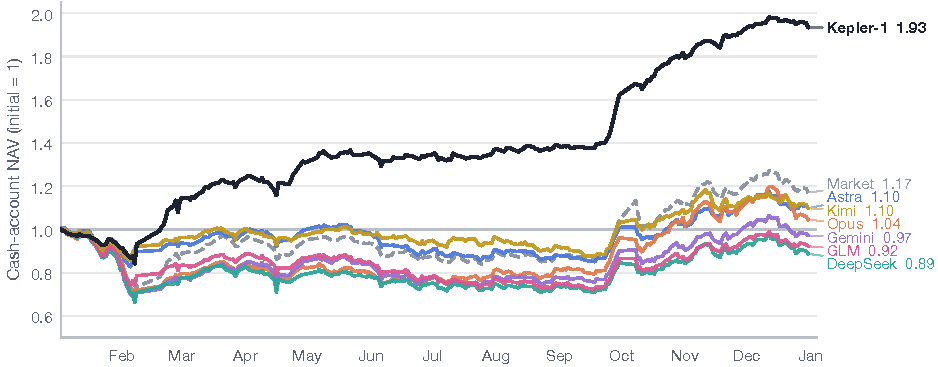
\includegraphics[width=\linewidth]{Figures/fig_nav.pdf}
        \caption{Out-of-sample cash-account NAV in 2024 for the six selected iterative strategies in Table~\ref{tab:main}, our closed-source reference Kelper-1, and the equal-weight market reference. All series use initial capital of 1. The market reference is gross of trading costs.}
        \label{fig:nav}
    \end{minipage}
\end{table*}

The highest-scoring model entry in Table~\ref{tab:main} is Opus with iterative research, at 31.9 points, followed by Astra at 30.3 and DeepSeek at 29.5. All remain below the professional reference, which scores 52.5. The separation is also visible in returns: Opus achieves 30.4\% ARR, compared with 88.3\% for Kelper-1.

Positive returns do not consistently translate into outperformance. Four of the six selected iterative strategies have positive ARR, but only Opus and DeepSeek exceed the market reference, by 13.3 and 1.9 percentage points, respectively. Astra earns 16.4\% and Kimi 9.8\%, both below the reference. Gemini and GLM lose money despite receiving research feedback. Among the five models with retained entries in both settings, all one-shot strategies underperform the market.

Research-period scores and assessment-period outcomes also differ. Astra has the highest research-period score among models, at 36.7, but ranks behind Opus and DeepSeek on the sealed period. Gemini's score falls from 24.6 to 4.0, while GLM's falls from 13.5 to 0.0. Risk adds another distinction: DeepSeek's selected strategy has a Sharpe ratio of 1.16 and a maximum drawdown of 7.9\%, compared with 0.92 and 31.1\% for Opus. The higher-return strategy therefore does not dominate on risk.

Figure~\ref{fig:nav} shows the corresponding cash-account NAV paths throughout 2024.

\subsection{Effects of Research Feedback}
\label{sec:feedback_effect}
\label{sec:e2}

Iterative research improves the selected overall score for all five models with results in both settings. Excess ARR improves for four, with gains ranging from 7.5 percentage points for GLM to 39.0 for DeepSeek. Gemini is the exception: its score rises from 0.0 to 10.2, but its excess ARR falls by 4.3 percentage points.

To examine the role of performance feedback, we compare full feedback with an \textbf{errors-only} control for Astra and DeepSeek. Both conditions use the same research budget and evaluation rules. The control withholds performance metrics and score-derived labels while retaining execution status, errors, candidate identifiers, and remaining-budget information. Models can still repair their code, revise strategies, and select a completed candidate. Table~\ref{tab:feedback} compares the retained control entries with the full-feedback entries in Section~\ref{sec:main}.

\begin{table*}[t]
\centering
\footnotesize
\caption{Full performance feedback versus errors-only feedback. Each row reports one selected iterative strategy. ARR, excess ARR, and RankIC refer to 2024. Tokens are total model tokens consumed during research, in thousands. The selected Astra control is one of three completed controls tied at an overall score of zero.}
\label{tab:feedback}
\setlength{\tabcolsep}{6pt}
\begin{tabular}{@{}llrrrrr@{}}
\toprule
Model & Feedback & Overall & ARR (\%) & Excess (pp) & RankIC & Tokens (k) \\
\midrule
\ModelAstra & Full & 30.3 & 16.4 & $-0.7$ & 0.0462 & 95.7 \\
 & Errors only & 0.0 & $-6.5$ & $-23.5$ & 0.0018 & 50.3 \\
\midrule
\ModelDeepSeek & Full & 29.5 & 18.9 & +1.9 & 0.0494 & 418.2 \\
 & Errors only & 0.0 & $-3.1$ & $-20.2$ & $-0.0044$ & 155.1 \\
\bottomrule
\end{tabular}
\end{table*}


Both selected errors-only strategies score zero. Full-feedback entries achieve higher excess ARR by 22.9 percentage points for Astra and 22.0 for DeepSeek, alongside RankIC values of 0.0462 and 0.0494 rather than values near zero. The other two completed Astra controls also have negative excess returns.

The selected full-feedback attempts also use more of the available research budget. Astra evaluates four candidates instead of one, and DeepSeek five instead of three, with higher token consumption in both cases. These comparisons measure feedback-driven research under a common budget, including the additional computation used during revision.

\subsection{Predictive Signal versus Portfolio Outcome}
\label{sec:signal_vs_portfolio}

Strong signal statistics do not guarantee a strong portfolio. In the iterative track, all five models reach similar 2024 RankIC (0.029--0.049), yet their 2024 excess returns span 38 percentage points, from $+13.3$ to $-24.9$. The two models with the \emph{highest} in-sample RankIC, \ModelGemini\ (0.064) and \ModelGLM\ (0.056), produce the \emph{worst} 2024 portfolios. Their long--short Sharpe ratios fall to zero or below. \ModelClaudeOpus\ has the lowest 2024 RankIC of the five (0.029) but the best portfolio and a long--short Sharpe of 1.51.

RankIC measures how well a strategy orders the whole market. The portfolio depends only on the top 75 stocks, and on whether they can actually be bought and held under price limits. A model that optimizes average correlation can improve the ordering of thousands of uninteresting stocks while leaving the head of the ranking no better than chance. This is why \BenchmarkName\ scores signal and portfolio terms jointly, and why the geometric mean in Equation~\eqref{eq:quality} requires every term to be positive.

\subsection{Effect of Reasoning Effort}
\label{sec:effort}

\begin{figure}[t]
    \centering
    \figorph{Figures/fig_effort.pdf}{\linewidth}{Reasoning effort}
    \caption{Effect of reasoning effort. Total score and tokens used for each model at each reasoning setting. \ph{Results pending.}}
    \label{fig:effort}
\end{figure}

Reasoning effort is the main inference-time setting that participants control. For each model whose provider exposes a working control, we run both tracks at a low and a high setting, in addition to the default, under the same suite and budget. Providers control reasoning in different ways: discrete effort levels, explicit thinking budgets, or an on/off switch. Some models cannot vary it at all. We use each provider's native control and report the reasoning tokens actually consumed.

\phtext{Results pending: per-model findings on whether more reasoning improves the committed strategy, how it changes token use and therefore $E$, and whether it helps one-shot more than iterative research.}

\subsection{What Happens During Research}
\label{sec:process}

We compare the first executable candidate of each completed iterative run with the strategy it finally commits to. Eight of nine runs improve their in-sample excess return over that trajectory, by 10.6 percentage points on average. No run commits to its first candidate, and six commit to the candidate with the best in-sample result. Models therefore use feedback actively and select greedily on the research window. Because only the committed strategy is assessed on 2024, this improvement is in-sample progress. Section~\ref{sec:main} shows that it transfers unevenly.

\begin{figure}[t]
    \centering
    \figorph{Figures/fig_tokens_vs_score.pdf}{\linewidth}{Tokens vs score}
    \caption{Tokens used versus total score for all completed runs. Official runs are highlighted.}
    \label{fig:tokens}
\end{figure}

Token use and score are only loosely related (Figure~\ref{fig:tokens}). \ModelAstra\ reaches 30.29 with 96k tokens, while \ModelGemini\ and \ModelGLM\ spend about 370k tokens for scores of 10.22 and 4.05. \ModelClaudeOpus\ and \ModelDeepSeek\ spend 320k and 418k for the top two out-of-sample scores. Spending more of the budget helps only when the model can turn feedback into better candidates.

\subsection{Reliability}
\label{sec:reliability}

\begin{table}[t]
\centering
\small
\caption{Run outcomes per model and track in the main campaign (snapshot of 18 October 2026). Attempts exclude runs cancelled by the operators because of platform or model-provider incidents, and runs still in progress. A completed run has a frozen strategy with a sealed assessment.}
\label{tab:attempts}
\begin{tabular}{@{}lrrrrrr@{}}
\toprule
 & \multicolumn{3}{c}{One-shot} & \multicolumn{3}{c}{Iterative} \\
\cmidrule(lr){2-4}\cmidrule(l){5-7}
Model & Att. & Done & Failed & Att. & Done & Failed \\
\midrule
\ModelClaudeOpus & 10 & 3 & 7 & 3 & 2 & 1 \\
\ModelAstra & 3 & 3 & 0 & 3 & 3 & 0 \\
\ModelDeepSeek & 3 & 3 & 0 & 1 & 1 & 0 \\
\ModelGemini & 4 & 3 & 1 & 2 & 2 & 0 \\
\ModelGLM & 3 & 1 & 2 & 1 & 1 & 0 \\
\ModelKimi & 7 & 2 & 5 & 1 & 0 & 1 \\
\bottomrule
\end{tabular}
\end{table}


Completing a research run is itself a capability. Table~\ref{tab:attempts} reports all attempts in the main campaign, excluding runs cancelled because of platform or provider incidents. Failure rates differ sharply by model. Here a failure means the run produced no valid committed strategy: an invalid proposal, a strategy that fails during execution, or a harness protocol failure.
\begin{itemize}[leftmargin=*,itemsep=1pt]
    \item \ModelAstra\ and \ModelDeepSeek\ completed every attempt.
    \item \ModelClaudeOpus\ failed 7 of 10 one-shot attempts.
    \item \ModelKimi\ failed 5 of 7 one-shot attempts and its only iterative attempt.
\end{itemize}
\ModelKimi's failures occurred through a third-party relay and its runs through the official API are pending. \ph{Failure breakdown by cause pending.} A model that cannot reliably produce an executable strategy in one pass has a lower expected score in practice than its best run suggests.

\phtext{Stability across repeated runs of the same model and track is analyzed separately.}
